\chapter{An Interactive 3D Simulation Engine}
\label{ch:engine}

\section{Goals and Architecture}

The statistical simulator answers questions with tables and the Gazebo world
answers integration questions, but neither lets a person \emph{watch} the
pipeline think. The project therefore built its own interactive 3D simulation
engine, which runs in a web browser (Fig.~\ref{fig:eng:overview}). Its
requirements were that the real pipeline makes every decision; that rovers
move with correct differential-drive kinematics, smoothly and without ever
colliding; that links follow the rovers every frame and show what is kept,
what is a candidate, what has stretched out of range and where data flows;
that every parameter is tunable live; that the pipeline is compared honestly
against baselines it beats; and that the scene stays fast at any fleet size,
with orbit controls and a game-style map of every rover.

\begin{figure}[htbp]
\centering
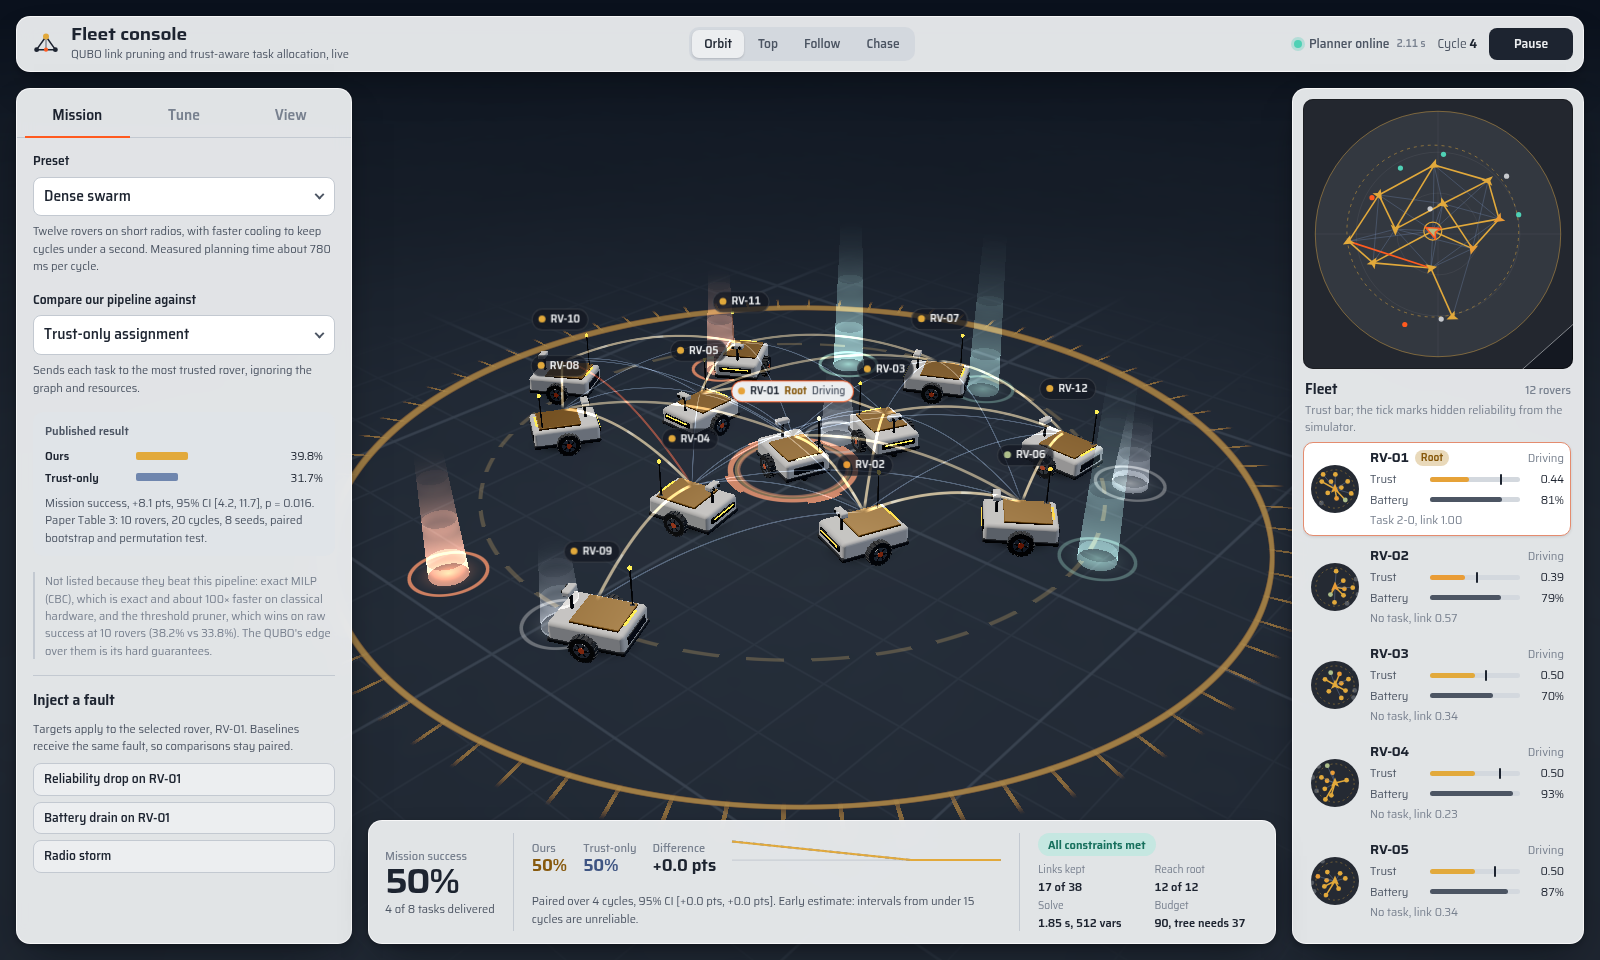
\includegraphics[width=0.92\linewidth]{figures/engine-overview.png}
\caption{The engine with the twelve-rover \emph{Dense swarm} preset: mission
controls (left), the 3D scene with kept links and task beacons (centre), the
overview map and per-rover radars (right), and the live comparison against
trust-only assignment (bottom).}
\label{fig:eng:overview}
\end{figure}

Responsibilities are split along one narrow interface. The browser owns time,
motion and rendering; a planner service, written in Python around the
unchanged closed-loop simulator, owns every decision. Once per planning cycle
the browser sends the rovers' live positions and the current parameters, and
the service runs one pipeline cycle in which those positions replace the
simulator's random walk, returning kept links, trust, assignments, task
outcomes and diagnostics. Parameter limits, presets and the comparison
catalogue live in one configuration document read by both sides, so they can
never disagree about what is valid. Each parameter carries a \emph{scope}:
fleet size and seed restart the mission, planner parameters apply from the
next cycle without losing learned trust, and speed, time scale and cycle
interval apply instantly (Table~\ref{tab:eng:params}).

\begin{table}[htbp]
\centering
\caption{Tunable parameters, their ranges and scopes.}
\label{tab:eng:params}
\footnotesize
\begin{tabular}{@{}l l l | l l l@{}}
\toprule
Parameter & Range & Scope & Parameter & Range & Scope \\
\midrule
rovers & 2--16 & session & annealer restarts & 2--6 & planner \\
scenario seed & 0--99\,999 & session & cooling rate & 0.980--0.999 & planner \\
cruise speed & 0--1.0 m/s & client & tasks per cycle & 1--4 & planner \\
time scale & 0.25--3$\times$ & client & exploration & 0--50\% & planner \\
radio range & 1.5--9 m & planner & trust memory $\alpha$ & 0.10--0.95 & planner \\
packet loss & 0--60\% & planner & reliability drift & 0--0.10 & planner \\
links per rover & 1--6 & planner & planning cycle & 0.8--6 s & client \\
link budget & 0--160 units & planner & & & \\
\bottomrule
\end{tabular}
\end{table}

\subsection{The Planner Service}

Each browser mission owns a planner \emph{session}. Alongside the primary
simulator run three \emph{paired followers}, one per assignment baseline
(trust-only, random, no-graph), created with the same seed and copying the
primary's kept links every cycle, so they differ from it \emph{only} in the
assignment policy; because they run from the start, a baseline chosen
mid-mission is still paired from the same initial state. For a solver
comparison, the exact Q matrix that the primary's annealer just solved, with
the same warm start, is handed to the chosen sampler. Faults are applied to
every arm. The service validates every field against the configuration
contract, answers ``busy'' rather than queueing, and evicts the longest-idle
session when full; the browser keeps exactly one request in flight, so a slow
solve stretches the cadence instead of piling up requests, and an answer for
an old fleet can never be applied to a new one.

The presets of Table~\ref{tab:eng:presets} were chosen by measurement. During
calibration a single annealer restart sent solvable instances to the
keep-all fallback (the restart-floor defect of Section~\ref{sec:sol:ladder}),
so every preset uses at least two.

\begin{table}[htbp]
\centering
\caption{Presets and their measured planner time per cycle.}
\label{tab:eng:presets}
\small
\begin{tabularx}{\linewidth}{@{}l r X r@{}}
\toprule
Preset & Rovers & Character & Cycle \\
\midrule
Field survey & 8 & balanced radio budget, the everyday setting & 680~ms \\
Rapid response & 6 & fast rovers, one-second planning cycle & 280~ms \\
Relay corridor & 10 & long radios; the QUBO trims a dense mesh & 750~ms \\
Dense swarm & 12 & short radios, faster cooling & 780~ms \\
Full fleet & 16 & the maximum fleet size & 1420~ms \\
Hostile radio & 8 & heavy packet loss, drifting reliability & 250~ms \\
Tight constraints & 10 & two links per rover, small budget & 140~ms \\
\bottomrule
\end{tabularx}
\end{table}

\section{The Motion Engine}

\subsubsection{Fixed step and interpolation} Motion is simulated at
$\Delta t=1/120$~s, independent of the display rate. Each frame adds its real
elapsed time (capped at 0.1~s, with a backlog cap of forty steps, so a stalled
tab cannot trigger a burst of catch-up work) to an accumulator, advances by
whole steps, and draws an interpolation between the last two steps with weight
$\alpha=\text{accumulator}/\Delta t$. Headings are interpolated along the
shorter arc, $\psi_0+\alpha\,\mathrm{wrap}(\psi_1-\psi_0)$, so a heading that
crosses $\pm\pi$ is never drawn spinning the long way round.

\subsubsection{Exact arc integration} The ground plane is spanned by $x$ and
$z$, and a rover with heading $\psi$ faces the direction
$(\cos\psi,\sin\psi)$, so a positive yaw rate is a right turn. For constant $v$ and $\omega$ over one step the rover
follows a circular arc exactly, whose chord has length
$v\Delta t\,\mathrm{sinc}(\omega\Delta t/2)$ along the mean heading:
\begin{equation}
\begin{aligned}
\begin{pmatrix}x'\\z'\end{pmatrix}&=\begin{pmatrix}x\\z\end{pmatrix}
+v\Delta t\,\mathrm{sinc}\!\left(\tfrac{\omega\Delta t}{2}\right)
\begin{pmatrix}\cos(\psi+\omega\Delta t/2)\\ \sin(\psi+\omega\Delta t/2)\end{pmatrix},\\
\psi'&=\mathrm{wrap}(\psi+\omega\Delta t),
\end{aligned}
\label{eq:eng:arc}
\end{equation}
with $\mathrm{sinc}$ evaluated by its Taylor series near zero. Unlike an Euler
step, this update does not drift on curves.

\subsubsection{Wheels and limits} Because a positive yaw rate turns right,
the left wheel runs on the outside of the arc:
$v_L=v+\omega L_w/2$ and $v_R=v-\omega L_w/2$, Eq.~\eqref{eq:gz:diffdrive}
rewritten for the mirrored yaw convention. An early prototype kept the Gazebo
signs in this frame and spun the wheels backwards on every turn; a test that
integrates each wheel's contact point and compares its path with
$v_{L,R}\Delta t$ now pins the relation. Commands respect acceleration
(0.9~m/s$^2$), braking (1.8~m/s$^2$), yaw rate (1.8~rad/s) and rim speed
(1.25~m/s). An over-fast command is scaled as
$(v,\omega)\leftarrow\kappa(v,\omega)$ with
$\kappa=\min\bigl(1,v_{\max}/\max(|v_L|,|v_R|)\bigr)$, which preserves the
curvature $\omega/v$: the rover follows the same arc, only slower.

\subsubsection{Steering} Each rover drives towards its task site or, when
idle, a patrol point. The desired heading adds to the goal direction a
repulsion from rovers within a sensing radius, weighted by
$\bigl((S-d)/(S-2R_b)\bigr)^2$; a \emph{keep-right} term for rovers ahead, so
two rovers meeting head-on veer the same way and pass; an inward push at the
arena edge; and, for idle rovers, a pull towards the nearest neighbour when it
drifts beyond 85\% of the radio range, which keeps the mesh connected. Speed
scales with the squared cosine of the heading error, and near $\pm\pi$ the
previous turn direction is held so the rover does not oscillate.

\subsection{Collision Safety}

Each footprint is enclosed in a circle of radius $R_b=0.62$~m, so collision
freedom means every pair of centres stays at least $2R_b$ apart.

\begin{proposition}[Sequential commits never overlap]
Rovers are updated one at a time. Rover $i$'s proposed translation is accepted
only if, for every other rover $j$ at its \emph{current} position, the new
distance satisfies $d'_{ij}\ge2R_b$ or $d'_{ij}\ge d_{ij}$; otherwise $i$ only
rotates in place. Then after every step
$d_{ij}^{\text{new}}\ge\min(2R_b,d_{ij}^{\text{old}})$ for every pair.
\end{proposition}

\begin{proof}
For a pair $i<j$, rover $i$ is checked against $j$'s old position and rover
$j$, moving later, against $i$'s new position, so
\[
d(p_i',p_j)\ge\min\bigl(2R_b,d(p_i,p_j)\bigr),\qquad
d(p_i',p_j')\ge\min\bigl(2R_b,d(p_i',p_j)\bigr).
\]
Chaining the two gives the claim, and a rejected move leaves its inequality
trivially true. A rotation in place does not move the centre of a circle, so
it is always safe; the same argument keeps every rover inside the arena.
\end{proof}

The ``or no closer'' clause lets rovers that start too close separate instead
of locking. Safety alone can still freeze a crowd, so every two seconds a
rover that has gained less than 0.15~m towards its goal, or has been blocked
for more than 1.2~s, takes a \emph{detour} through a temporary waypoint about
$63^\circ$ off its goal direction, alternating sides on repeated attempts;
after five failed detours it abandons the errand. Rovers spawn by
deterministic dart throwing with spacing $2R_b+0.35$~m, falling back to a
hexagonal lattice that is guaranteed to hold the largest fleet. Tests drive
sixteen rovers at triple speed for 1\,800 frames without a single overlap and
check that a dense swarm keeps moving.

\section{The Renderer}

\begin{figure}[!htbp]
\centering
\begin{minipage}[b]{0.49\linewidth}
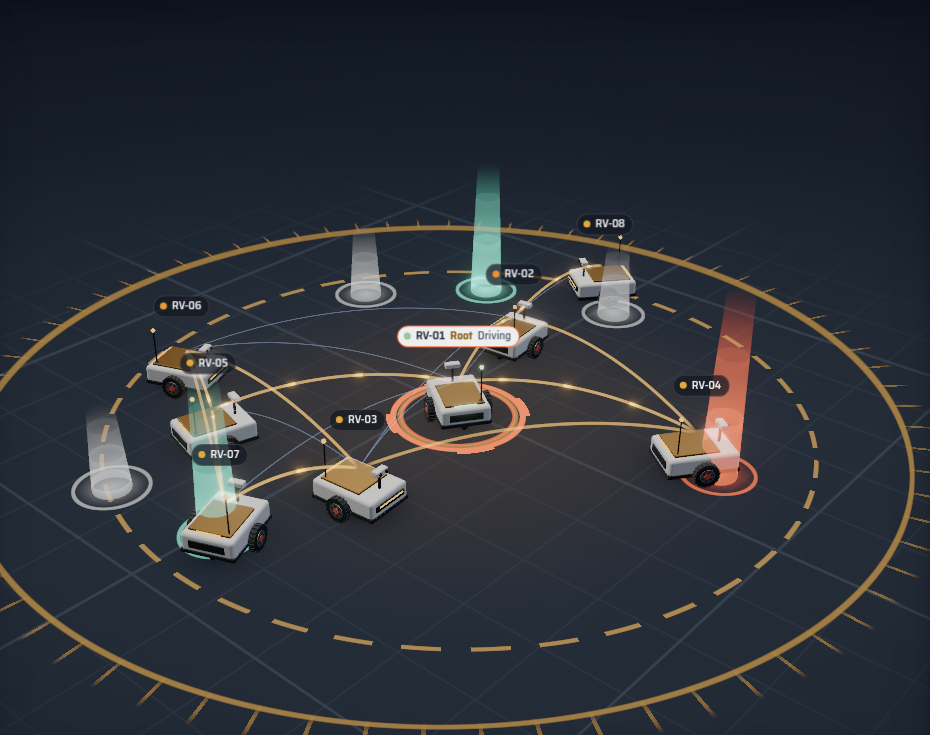
\includegraphics[width=\linewidth]{figures/engine-orbit.png}
\end{minipage}\hfill
\begin{minipage}[b]{0.49\linewidth}
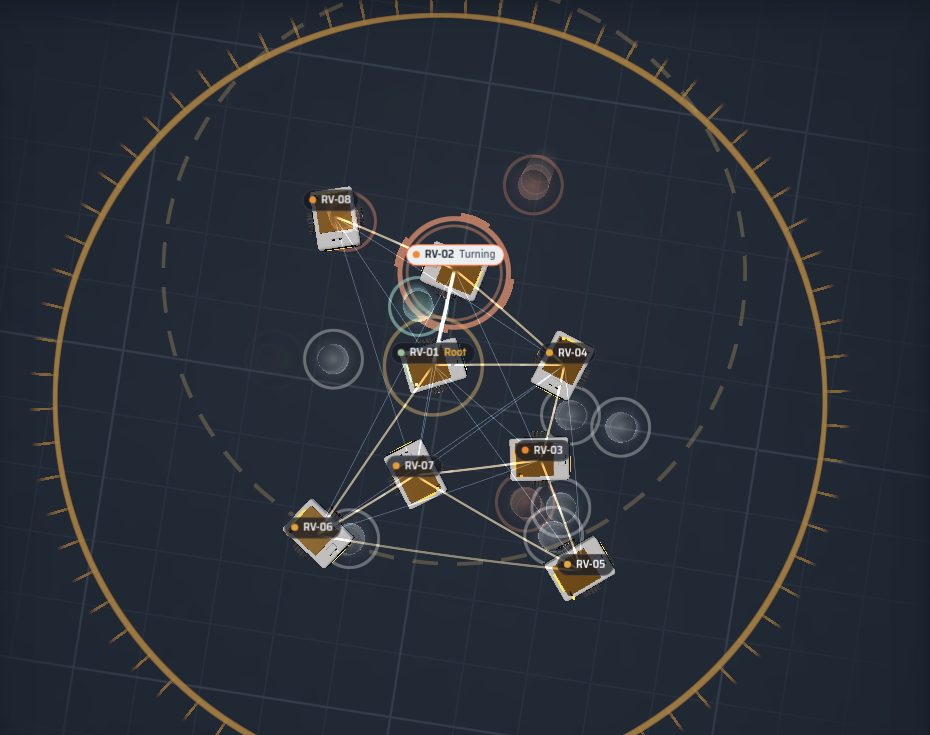
\includegraphics[width=\linewidth]{figures/engine-top.png}
\end{minipage}
\caption{The eight-rover \emph{Field survey} preset from the orbit camera
(left) and the top camera (right): gold kept links, faint candidates, task
beacons resolving to success (mint) or failure (orange), and the root's ring.}
\label{fig:eng:views}
\end{figure}


Figure~\ref{fig:eng:views} shows the default mission from the orbit and top
cameras. A naive scene creates one mesh per rover part and one line per link, so its
draw calls, each carrying fixed CPU-side driver overhead, grow with the fleet.
The engine instead renders every object class in one instanced draw call:
the whole scene costs \textbf{seven draw calls} whatever the fleet size: the
ground (one shader disc with grid, rim and fog), the ground markers (shadows,
selection ring, radio ranges and beacon pads as instanced quads), the rover
bodies (all parts merged into one geometry), the wheels (one geometry for both
sides of every rover), the status lights, the radio links (instanced arc
ribbons) and the task beacons. Eight rovers come to about 26\,000 triangles. Per-instance data lives in pre-allocated buffers written in place and
uploaded only over the range in use, so a frame allocates no memory.



\begin{figure}[htbp]
\centering
\begin{minipage}[b]{0.55\linewidth}
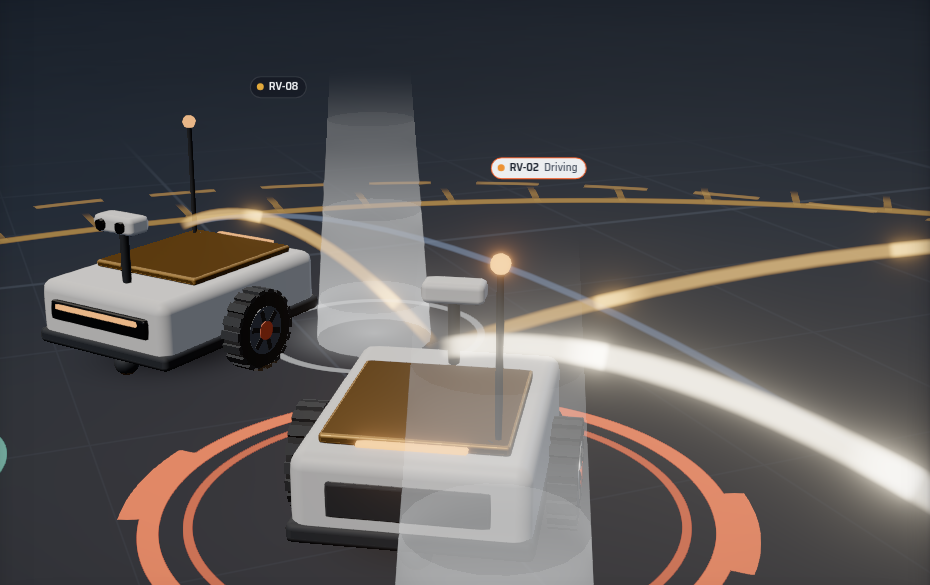
\includegraphics[width=\linewidth]{figures/engine-chase.png}
\end{minipage}\hfill
\begin{minipage}[b]{0.42\linewidth}
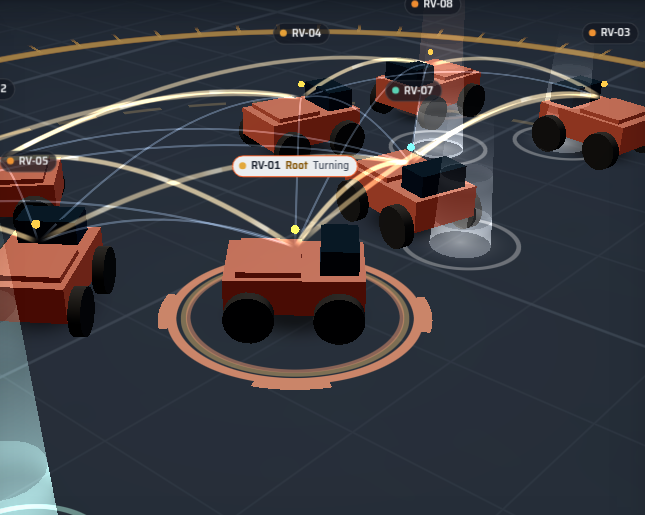
\includegraphics[width=\linewidth]{figures/engine-glb.png}
\end{minipage}
\caption[Left: chase camera behind the default rover (ceramic body, gold-foil deck, stereo camera, antenna light, treaded wheels with orange hubs).]{Left: chase camera behind the default rover (ceramic body, gold-foil
deck, stereo camera, antenna light, treaded wheels with orange hubs). Right: a
four-wheeled model imported from Blender, whose named wheels were detected and
spin with the fleet's kinematics.}
\label{fig:eng:chase}
\end{figure}

\subsubsection{The rover} The default rover reproduces the Gazebo model's
dimensions and adds detail that makes heading and motion readable
(Fig.~\ref{fig:eng:chase}). Parts of different colour and finish are merged
into one geometry by storing colour, roughness and metalness per vertex and
patching the standard physically based material to read them. Any rigid model
exported from Blender as binary glTF can replace it: the import validates the
file, centres and grounds it, rotates its forward axis onto the engine's,
scales its footprint to the collision circle, merges meshes per material, and
detects meshes named as wheels, which then spin at $v_{L,R}/r$ for their own
measured radius.

\subsubsection{Radio links} Each link is a camera-facing ribbon bent into a
shallow arc between two antennas, computed in a vertex shader so the CPU only
supplies end points. For a link from $A$ to $B$ of length $\ell$,
\begin{equation}
P(t)=A+t\,(B-A)+\hat y\,h\,4t(1-t),\qquad h=\mathrm{clamp}(0.08+0.06\,\ell,\ 0.1,\ 0.5),
\end{equation}
widened along the normalised cross product of $P'(t)$ and the direction to
the camera, with a horizontal fallback when the camera looks along the link.
Links are styled \emph{kept} (gold), \emph{candidate} (faint),
\emph{stretching} (flickering orange: kept, but out of range since the last
plan) or \emph{delivery path} (bright), and packets travel along kept links
towards the root in the widest-path tree.

\subsubsection{Ground and post-processing} The ground is one shader with an
anti-aliased grid, the arena rim and the same linear fog as the standard
materials. A post-processing chain adds anti-aliasing, bloom, filmic tone
mapping and a vignette in three quality tiers, and an adaptive monitor steps
down a tier when the frame rate falls. On one real GPU a screen-space
ambient-occlusion pass produced black frames, because it could not read the
multi-sampled depth buffer on that driver; the pass was removed, and a guard
now samples five pixels after start-up and steps down a tier if all of them
are black, which the ground and sky never are. A paused mission renders only
on demand.

\section{The Interface}

Four cameras are available, orbit, top-down, follow and chase, with damped
transitions that yield as soon as the user touches the controls. The right
column (Fig.~\ref{fig:eng:column}) is a game-style overview: a north-up map of
the whole arena with links, task sites, every rover as an arrow coloured by
trust, and the 3D camera's ground footprint, computed by intersecting the rays
through the screen corners with the ground; below it, each rover's card shows
a heading-up radar scaled to its radio range, its trust with a tick at its
hidden true reliability, its battery and its task. The left panel holds
presets, the comparison selector with the published reference result, fault
injection, the tuning sliders with graph-theory advisories, overlays, quality
tiers with live frame rate and draw calls, and model import.

\begin{figure}[htbp]
\centering
\begin{minipage}[c]{0.26\linewidth}
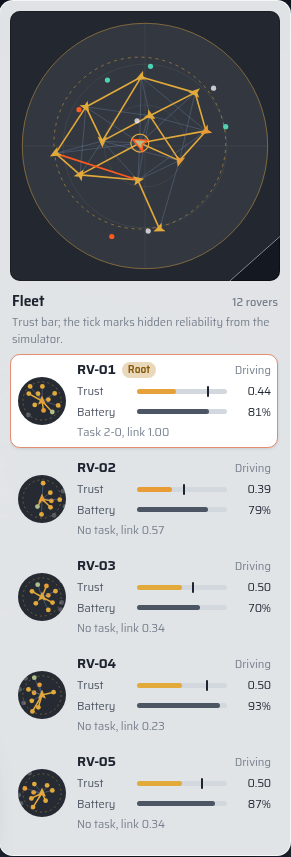
\includegraphics[width=\linewidth]{figures/engine-fleet-column.png}
\end{minipage}\hfill
\begin{minipage}[c]{0.7\linewidth}
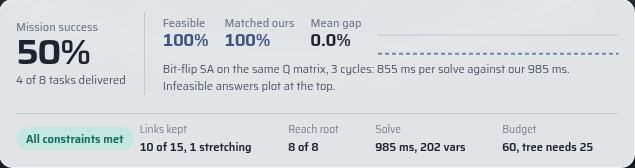
\includegraphics[width=\linewidth]{figures/engine-strip.png}\\[6pt]
\small Left: the overview map with the camera's view outline, and rover cards
with heading-up radars. Right: the mission strip during a live comparison with
bit-flip SA on the same Q matrix: feasibility, match rate, energy gap and the
planner's guarantee status.
\end{minipage}
\caption{Overview map, rover radars and the live comparison strip.}
\label{fig:eng:column}
\end{figure}

The comparison selector lists only baselines that the published results show
the pipeline beats (trust-only and random assignment, the no-graph readout
marked as not significant, and the four samplers), and directly beneath it
names the two methods that beat the pipeline, the exact MILP and the threshold
pruner. For assignment baselines the strip shows paired success rates, their
difference and a bootstrap confidence interval, with a warning while fewer
than fifteen cycles have been collected; for solver baselines it shows
feasibility, match rate, mean energy gap and time per solve. In one 22-cycle
run, bit-flip SA matched our optimum in 68\% of cycles with a mean gap of
1.7\%, in line with the offline benchmark. Short runs can go either way, and
the engine shows them as they are.

\section{Edge Cases and Verification}

Table~\ref{tab:eng:edge} lists the main edge cases and their treatment.

\begin{table}[htbp]
\centering
\caption{Edge cases handled by the engine.}
\label{tab:eng:edge}
\small
\begin{tabularx}{\linewidth}{@{}p{4.2cm}X@{}}
\toprule
Situation & Treatment \\
\midrule
Degree cap 1, three or more rovers & a spanning tree needs a node of degree 2, so connectivity is impossible; announced before the planner relaxes it \\
Degree cap 2 & only a chain through every rover (a Hamiltonian path) remains; relaxations announced \\
Budget below $n-1$ units & every link costs at least one unit, so it can never be met \\
Budget versus the live graph & shown next to the cheapest spanning tree of the live graph \\
No links in range & reported as such, never as an empty success \\
Angles near $\pm\pi$; zero yaw rate & short-arc interpolation, held turn direction; Taylor series for $\mathrm{sinc}$ \\
Stalled tab; bad frame times & 0.1~s frame cap, 40-step backlog cap, invalid deltas ignored \\
Malformed or stale planner data & invalid indices and values ignored; one request in flight; old-fleet answers aborted \\
Planner busy, full or offline & retry, idle-session eviction, or exponential back-off with a notice \\
GPU context lost; black post-processing & explanatory overlay; five-pixel guard steps down a tier \\
\bottomrule
\end{tabularx}
\end{table}

The motion mathematics is covered by seventeen property tests and the planner
service by nineteen tests (Chapter~\ref{ch:verify}). The engine was exercised
in a browser at desktop, laptop and phone widths, where the panels reflow into
one scrolling column.


